\documentclass{alex_bericht}
\usepackage{pdfpages}

\DeclareSIUnit\FU{F.U.}

\definecolor{MyBlue}{HTML}{0072B2}
\definecolor{MyOrange}{HTML}{D55E00}
\definecolor{MyRed}{HTML}{F00F0F}
\definecolor{MyGreen}{HTML}{20B312}

\usetikzlibrary{math, arrows.meta, calc, angles, quotes, arrows, shapes.geometric, decorations.pathmorphing, overlay-beamer-styles, patterns.meta}

\tikzset{
	partial ellipse/.style args={#1:#2:#3}{
		insert path={+ (#1:#3) arc (#1:#2:#3)}
	}
}

\tikzset{snake arrow/.style=
	{-Latex,
		decorate,
		decoration={snake,amplitude=.4mm,segment length=2mm,post length=1mm}},
}

\begin{document}
%Seiten ohne Kopf- und Fußzeile sowie Seitenzahl
\pagenumbering{Roman}
% !TeX root = Bericht.tex
% !TeX spellcheck = de_AT
\thispagestyle{empty}
\titlehead{\includegraphics[width=5cm]{logo.jpg}}
\title{Über das Aussehen von relativistisch ausdehnende Radioquellen}
\author{Alexander Helbok\thanks{\href{alexander.helbok@student.uibk.ac.at}{alexander.helbok@student.uibk.ac.at}}}
\date{\today}
\maketitle
\vfill 

%Inhaltsverzeichnis
{\hypersetup{linkcolor=black}
\clearpage
\tableofcontents

%Verzeichnis aller Bilder
%\listoffigures

%Verzeichnis aller Tabellen
%\listoftables}
\cleardoubleoddpage

\pagenumbering{arabic}
% !TeX root = Bericht.tex
% !TeX spellcheck = de_DE
\section{Einleitung}
\label{sec:einleitung}
In 60 Jahren kann sich das physikalische Weltbild stark verändern. Vor allem wenn man an die erste Hälfte des 20. Jahrhunder denkt, wo ein ganzer Teilbereich mit der Quantenmechanik neu aufgestellt wurde. Dennoch waren Physiker sich der Implikationen von Einsteins  Relativitätstheorie auch nach 60 Jahren noch nicht ganz bewusst. Wie die Welt bei relativistischen Geschwindigkeiten aussieht, kann man nur anhand mathematischer Formeln erahnen, so kontraintuitiv sind die Konzepte der SRT.

So geschah es, dass 1966 (61 Jahre nach Veröffentlichung der speziellen Relativitätstheorie), die starken Helligkeitsschwankungen von entfernten Radioquellen durch ein simples geometrisches Argument erklärt werden konnten. 
Das geometrische Argument trägt aber auch ein scheinbares Paradoxon mit sich, und zwar sich mit Übberlichtgeschwindigket ausdehnende Körper.

% !TeX root = Bericht.tex
% !TeX spellcheck = de_AT

\section{Problematik}
Der Bereich der Radioastronomie ist in den 30er Jahren aufgekommen und hat Astronomen ein neues Paar Augen geöffnet. Während optische Lichtwellen leicht abgeschirmt werden (durch Staub und Gas), können Radiowellen aufgrund ihrer großen Wellenlänge (und niedriger Energie) sich viel weiter fortpflanzen, ohne starke Verluste zu erleiden. Deshalb können mit Radioteleskopen Objekte beobachtet werden, die große Entfernungen besitzen.

Mitte der 60er Jahre waren genug Radiodurchmusterungen des Himmels durchgeführt, um die ungewöhnlichen beobachteten Objekte zu klassifizieren. Im Optischen erscheinen diese entweder gar nicht oder nur sehr schwach und punktförmig, wie Sterne. Im Radiobereich, strahlen sie sehr stark und man erkennt zum Teil räumliche Ausdehnungen. Hinzu  kommt, dass das Spektrum das eines schwarzen Strahlers gar nicht ähnelt und Spektrallinien zu sehen sind, die hohe Rotverschiebungen und somit hohe Entfernungen andeuten. Diese Objekte wurden aufgrund ihrer optischen Ähnlichkeit mit Sternen quasi-stellare-Objekte, kurz QSO oder Quasare, getauft. 

Was Quasare zu einzigartigen (und physikalisch äußerst problematischen) Objekten macht, sind folgende drei Beobachtungen:
\begin{enumerate}
	\renewcommand{\labelenumi}{\arabic{enumi})}
	\item Falls die Rotverschiebung der Spektrallinien (\( z > 0.1\)) der Expansion des Universums zugeschrieben werden kann, dann haben Quasare Entfernungen von über \( 500 \unit{Mpc} \).
	\item Der gemessene Fluss von Quasaren ist hoch.
	\item Der Strahlungsfluss von Quasaren vervielfacht sich innerhalb von Tagen.
\end{enumerate}

Aus Beobachtungen 1 \& 2 kann man sich unter der Annahme von Isotropie die gesamte Strahlungsleistung ausrechnen und man erhält Werte, welche die der Milchstraße um ein Vielfaches übersteigt. Das ist an sich nicht problematisch, da die beobachteten Galaxien großer als die Milchstraße sein könnten und daher natürlicherweise stärker Strahlen. Aus der Periode der Helligkeitsschwankungen (Beobachtung 3) kann man die Größe der strahlenden Region von oben abschätzen. Nachdem die für die Strahlung verantwortliche Region in kausalen Kontakt stehen muss und sich Informationen höchstens mit Lichtgeschwindigkeit fortpflanzen können, folgt, dass deren Ausdehnung nicht viel größer sein kann, als die Lichtlaufzeit. \autocite{comins}

Drastische Helligkeitsschwankungen lassen sich zum Beispiel am Quasar 3C 273 beobachten. Dieser ist der optisch Hellste am Nachthimmel und gehört zu den Nächstgelegenen bei einer Rotverschiebung von \( z = 0.158 \) \autocite{3c273}. Das macht ihn zu einem sehr interessanten Objekt und es wird bis heute noch extensiv von Astronomen beobachtet. In \autoref{fig:quasarflux} sind Flussmessungen des Quasars 3C 273 in verschiedenen Wellenlängen dargestellt.

\begin{figure}[H]
	\centering
	\begin{subfigure}{.45\textwidth}
		\centering
		\includegraphics[width=\linewidth]{oldflux}
	\end{subfigure}%
	\begin{subfigure}{.55\textwidth}
		\centering
		\includegraphics[width=\linewidth]{newflux}
	\end{subfigure}
	\caption{Links ist der gemessene Fluss auf die Zeit aufgetragen. An Beobachtungen die bei gleichen Wellenlängen durchgeführt wurden, sind Geraden angepasst worden. In der rechten Abbildung ist der gemessene Fluss des gleichen Quasars auf die Wellenlänge für drei unterschiedliche Messreihen (farblich hervorgehoben) aufgetragen. Graphiken stammen aus \autocite{oldflux} und \autocite{newflux}.}
	\label{fig:quasarflux}
\end{figure}

In der Linken Abbildung aus 1965 \autocite{oldflux} sind Flussmessungen bei verschiedenen Wellenlängen zu unterschiedlichen Zeitpunkten angegeben. Die gemessene Flussdichte ist mit Fehlerbalken auf den Beobachtungszeitpunkt aufgetragen, die vertikale Achse ist nicht kontinuierlich, da der Fluss in unterschiedlichen Spektralbändern der gleiche ist diese Ansicht gewählt wurde, um die Spektralbänder unterscheidbar zu machen. Auf Messungen aus dem gleichen Spektralband wurden lineare Regressionen angewendet und die erhaltenen Geraden sind strichliert dargestellt. Bei \( 3.75 \unit{cm} \) haben die Erstautoren keine Daten aufgenommen, die durchgezogene Linie stammt aus \autocite{other} und wurde inkludiert, da sie ein ähnliches Verhalten wie die gesammelten Daten zeigt.

In der rechten Abbildung aus 2020 \autocite{newflux} ist die Flussdichte auf die Wellenlänge aufgetragen, wobei drei farblich unterscheidbare Kurven drei Messungen aus 2013 bis 2015, mit jeweils einem Jahr Abstand, darstellen. 

Man erkennt in beiden Graphiken, dass die Helligkeit sich verändert, links nimmt sie zu während sie rechts abnimmt. Um die Größe der Region abzuschätzen, die in 3C 273 für die Stahlung verantwortlich ist, muss man streng genommen eine Trendumkehr beobachten (halbe Periode der Schwankung). In \autoref{fig:quasarflux} ist das nicht der Fall, die Größenordnung lässt sich aber auf Lichtjahre fixieren, da zwischen 1960 und 2015 offensichtlich eine Umkehr der Helligkeit stattgefunden hat. 

Stimmen diese drei Aussagen/Beobachtungen, die zu Beginn genannt wurden, haben wir es also bei Quasaren mit Objekten zu tun, deren Strahlungsregion die Größenordnung des Sonnensystems hat (Aussage 1) und ein Vielfaches der Milchstraße strahlt (Aussage 1 \& 2).  Das ist äußerst problematisch, da kein physikalischer Prozess bekannt ist, der eine solche Energiedichte erzeugen kann. Eine der Beobachtungen

\section{Lösungsvorschlag}
Eine erhöhte Flussdichte erhält man entweder durch einen erhöhten gesamten Energieausstoß oder durch eine vergrößerte Oberfläche, welche mit der gleichen Energiedichte strahlt. Prozesse, die den Energieausstoß auf den Größenordnungen wie es bei Quasaren beobachtet wird, so schnell erhöhen, sind schwer.

Eine Vergrößerung der strahlenden Oberfläche kann z.B. durch Explosionen leicht argumentiert werden, reicht aber aus klassischer Sicht nicht aus, um die Beobachtungen zu erklären. Betrachtet man dieses Argument aber relativistisch, sieht das ganze aber anders aus.

1966 hat Martin Rees folgendes vorgeschlagen \autocite{rees}:
Betrachte eine Explosion, welche sich sphärisch vom Mittelpunkt \( S \) gleichförmig mit der Geschwindigkeit \( v \) ausbreitet. Im klassischen Regime \( v \ll c \) erscheint die sich ausbreitende Oberfläche für einen Beobachter \( O \) im Abstand \( R \ll vt \) kreisförmig (2D Projektion). Der Radius des Kreises nach der Zeit \( t \) (\( t \) wird ab dem Zeitpunkt gemessen, an dem die Explosion in \( O \) beobachtet wird) ist dabei \( r = vt \), und der Winkeldurchmesser beträgt \( \theta = 2\arctan(\tfrac{vt}{R}) \approx 2\tfrac{vt}{R} \).

\begin{figure}[H]
	\centering
	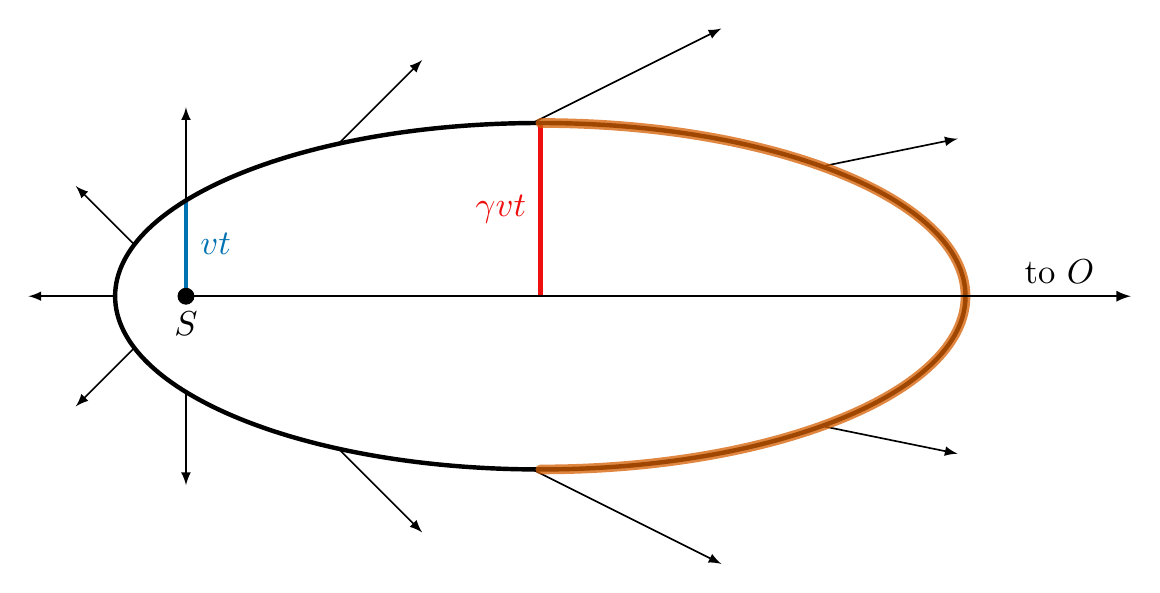
\begin{tikzpicture}[every node/.style={scale=1.25}, scale=2]		
		\coordinate (S) at (-2.5, 0);
		
		\draw[-latex, semithick] (S) -- (-3.5, 0);
		
		\draw[-latex, semithick] (S) -- (-3.2, 0.7);
		\draw[-latex, semithick] (S) -- (-3.2, -0.7);
		
		\draw[-latex, semithick] (S) -- (-2.5, 1.2);
		\draw[-latex, semithick] (S) -- (-2.5, -1.2);
		
		\draw[-latex, semithick] (S) -- (-1, 1.5);
		\draw[-latex, semithick] (S) -- (-1, -1.5);
		
		\draw[-latex, semithick] (S) -- (0.9, 1.7);
		\draw[-latex, semithick] (S) -- (0.9, -1.7);
		
		\draw[-latex, semithick] (S) -- (2.4, 1);
		\draw[-latex, semithick] (S) -- (2.4, -1);
		
		
		\draw[fill=white] (-0.25,0) ellipse (2.7 and 1.1);
		
		\draw[MyBlue, line cap=round, ultra thick] (S) -- (-2.5, 0.6) node [right, pos=0.55] {\( v t \)};
		\draw[MyRed, ultra thick] (-0.25, 0) -- (-0.25, 1.1) node [left, pos=0.5] {\( \gamma v t \)};
		
		\draw[ultra thick] (-0.25,0) ellipse (2.7 and 1.1);
		
		\draw[line width=3.5, MyOrange, opacity=0.75, line cap=round] (-0.25,0) [partial ellipse=-90:90:2.7 and 1.1];
		
		\draw[fill] (S) circle (0.05cm) node [below, yshift=-1] {\( S \)};
		
		\draw[-latex, thick] (S) -- (3.5, 0) node [above left, pos=0.975] {to \( O \)};
	\end{tikzpicture}	
	\caption{Wird eine sphärische Expansion bei relativistischen Geschwindigkeiten mit Ursprung \( S \) im Punkt \( O \) beobachtet, so erscheint diese nicht mehr rund, sondern elliptisch, mit \( S \) in einem Fokuspunkt. Die kleine Halbachse ist rot markiert und beträgt \( \gamma vt \). Ist das Ellipsoid optisch dick, sieht der erreicht nur das orange hinterlegte Segment den Beobachter.}
	\label{fig:superlum}
\end{figure}

Breitet sich die Explosion aber mit relativistischen Geschwindigkeiten aus \( v \sim c \) stimmt das klassische Bild nicht mehr. Aufgrund der Endlichkeit der Lichtgeschwindigkeit, wird in \( O \) kein \blockquote{Snapshot} der Explosion beobachtet, das Licht, welches Gleichzeitig eintrifft und somit das gesehene Bild erzeugt, wurde an unterschiedlichen Orten der Explosion zu verschiedenen Zeiten losgeschickt. Die Expansion erscheint also nicht mehr perfekt sphärisch, sondern wie ein Ellipsoid mit dem Ursprung der Explosion \( S \) in einem der Fokuspunkte (siehe \autoref{fig:superlum}). Normalkomponenten bleiben nach Lorentz-Transformationen in der speziellen Relativitätstheorie unverändert, weshalb der semi-latus rectum (in blau aufgetragen) mit \( vt \) dem klassischen Bild gleicht. Ist das beobachtete Objekt optisch dick, erreicht kommen in \( O \) nur Photonen aus der orange hinterlegten Region an. Die Expansion erscheint als Projektion also wieder kreisförmig, aber ist der Radius um einen Faktor \( \gamma = \left( 1-\tfrac{v^2}{c^2} \right)^{-1/2} \) gestreckt, wobei \( \gamma \) hier der Lorentzfaktor ist. Das Objekt scheint sich also schneller auszubreiten als es das tatsächlich tut.	

Den gesamten beobachteten Fluss erhält man, indem über die Oberfläche des Ellipsoids integriert wird. Das ist im Allgemeinen schwer, da die Strahlungscharakteristik zeitlich nicht konstant bleibt und das Licht, aus welchem der Ellipsoid konstruiert wird, nicht zur gleichen Zeit ausgesandt wurde. Nachdem die zu erklärenden Beobachtungen (siehe \autoref{fig:quasarflux}) im Radiobereich durchgeführt wurden, können wir uns hier auf diesen beschränken. Der Großteil davon ist Synchrotronstrahlung und wird von relativistischen geladenen Teilchen in einem Magnetfeld freigesetzt (was zum Modell einer relativistischen Expansion passt, falls diese von Elektronen getragen wird). Schränkt man das Spektrum nun weiter ein und beobachtet bei Frequenzen, bei welchen Selbstabsorption stattfindet, kann man die Form des gemessenen Spektrums abschätzen, da Selbstabsorption bei Synchrotronstrahlung einen Spektralindex von etwa \( 2.5 \) hat \autocite{spectral}. Daraus lässt sich der gesamte Strahlungsfluss berechnen und man findet, dass dieser im Vergleich zu einer statischen Quelle mit gleichem Winkeldurchmesser um einen Faktor \( \sim\sqrt{\gamma } \) größer ist \autocite{rees}.

Falls das Modell stimmt, muss es die damaligen Beobachtungen in \autocite{oldflux} erklären. Diese haben in einem Zeitraum von 3 Jahren eine Veränderung von 6 Flusseinheiten (\( \oldunit{\FU} \)) gemessen. In \autocite{rees} wird gezeigt, dass für eine Expansion mit \( \gamma = 5 \), der gemessenen Fluss in ebendiesem Zeitintervall um \( 15 \unit{\FU} \) zunimmt. Die dort getroffene Annahme von \( \gamma = 5 \) ist absolut legitim und das berechnete Ergebnis ist größer als der gemessene Wert, was das Modell unterstützt. 

Ein Nebeneffekt der relativistischen Betrachtung ist aber, dass die beobachtete Ausbreitungsgeschwindigkeit um den Lorentzfaktor \( \gamma \) erhöht ist. \( \gamma \) ist nach oben unbeschränkt, wodurch \( \gamma v > c \) möglich ist. Nachdem \( \gamma \) von der Geschwindigkeit abhängt, lässt sich diese Ungleichung in \( v > \tfrac{c}{\sqrt{2}} \approx 0.707c \) umschreiben. Solche Geschwindigkeiten sind absolut realistisch und wurden in Radioquellen auch beobachtet. 

Mittels Radiointerferometrie lassen sich auch in sehr großen Entfernungen Strukturen auflösen, sodass man zu Zeiten von Martin Rees bereits Komponenten außerhalb der Kernregion von Quasaren beobachtet hat, wobei diese Entfernungen von bis zu \( 10^6  \) Lichtjahren erreichen. Klassisch betrachtet bedeutet das, dass der Ursprung dieser Ausstöße älter als die Entfernung geteilt durch \( c \) sein muss. Im Falle von Quasaren ist das schwer nachzuvollziehen, da diese einen enormen Energieausstoß besitzen, der über Millionen von Jahren aufrechterhalten werden muss. Eine relativistische Betrachtung sagt aber, dass die Entfernung (über die Geschwindigkeit) um \( \gamma \) gestreckt ist, wodurch diese Komponenten weniger entfernt sind und das Alter der Radioquellen weniger problematisch wird.

Mittlerweile weiß man, dass relativistische Elektronen aus der Kernregion in entgegengesetzten Strahlen ausgestoßen werden, sogenannte kosmische Jets. Starke Magnetfelder sind für die Fokussierung der Strahlen und die hohe Synchrotronemission verantwortlich. Der Materiefluss ist zeitlich nicht konstant, wodurch der gemessene Fluss im Radiobereich abwechselnd zu- und abnimmt.  


% !TeX root = Bericht.tex
% !TeX spellcheck = de_AT
\section{Diskussion}
Das zu Beginn eingeführte Dilemma wurde von Martin Rees gelöst, indem die Helligkeitsfluktuationen nicht durch intrinsische physikalische Prozesse hervorgerufen werden, sondern durch rasch ausdehnende strahlende Oberflächen. Falls die Ausbreitungsgeschwindigkeit nahe der Lichtgeschwindigkeit ist, muss die spezielle Relativitätstheorie berücksichtigt werden, die eine Verzerrung des Bildes verursacht. Dieser Effekt reicht aus, um vorhandene Beobachtungen zu erklären.

Das Modell löst aber auch weitere Probleme. Einerseits stimmt die Abschätzung des Alters von Quasaren über dem Abstand der Materieausstöße nicht mehr, da die beobachtete Entfernung nicht der tatsächlichen entspricht. Andererseits liefert es eine Erklärung für messbare Überlichtgeschwindigkeit. Letzteres war in den 60er Jahren noch nicht aufgekommen, wurde aber in darauf folgenden Jahren beobachtet.


%%Literaturverzeichnis
\printbibliography

%\includepdf[noautoscale]{Unterschriften}

\end{document}
